\section{Methods}\label{sec:methods}

\subsection{Scope and implemented architecture}
We evaluated a reference implementation for structured pre-consultation using
synthetic patients. The objective was software verification: interchange of
clinical data, completion of the interview-to-write-back workflow, replacement of
model adapters, and concurrent operation. Diagnostic accuracy, triage accuracy,
clinical note quality, and comparisons with clinicians were outside scope.

The implementation comprises a Vue patient interface, a clinician interface,
a FastAPI backend, a local retrieval component, and a FHIR server
(Fig.~\ref{fig:architecture}). The patient interface uses an invitation exchanged
for a scoped session cookie. The clinician launcher binds the patient and visit
before the interview. SMART launch is a separate integration surface; it is not
equivalent to exchanging the patient invitation. Experiment instances use an
isolated SQLite database and an explicit loopback development authorization
bypass. Consequently, these runs do not establish production authorization or
institutional security assurance.

\begin{figure}[t]
\centering
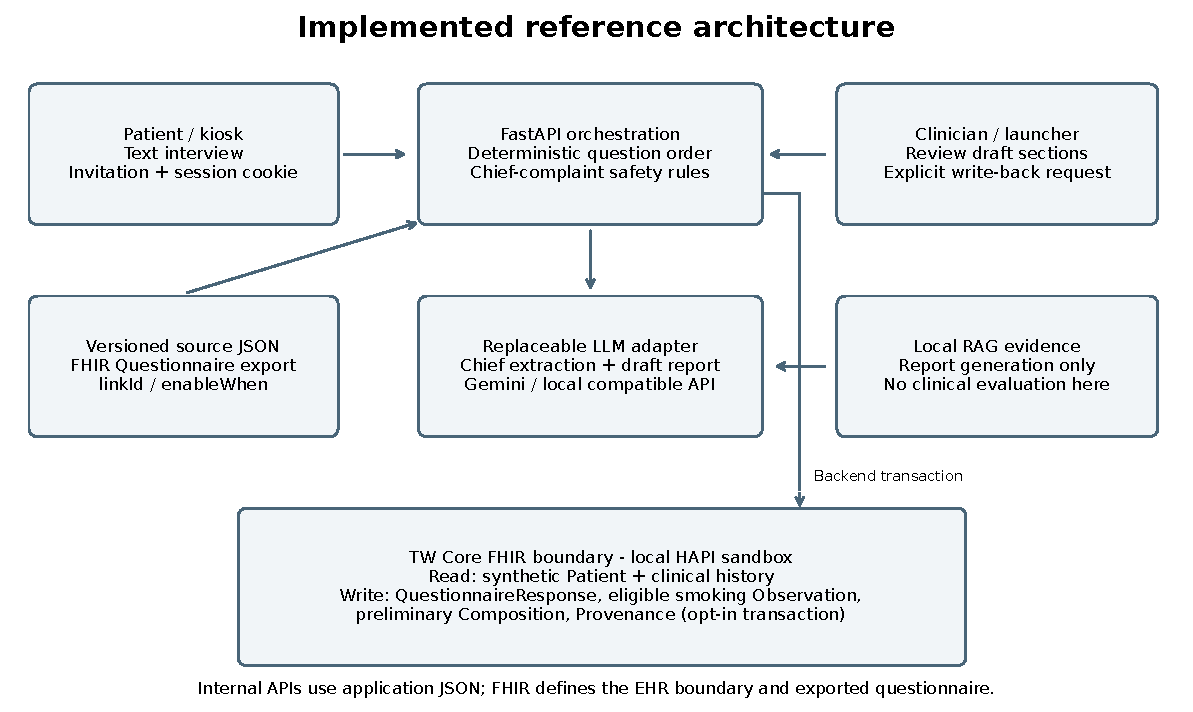
\includegraphics[width=\textwidth]{figures/fig1_architecture.pdf}
\caption{Implemented modules and data boundaries. The running questionnaire
engine consumes versioned application JSON; an encoder exposes a corresponding
FHIR Questionnaire. Internal application APIs are JSON contracts, whereas the
EHR boundary uses FHIR. Arrows do not imply a universal FHIR-native internal bus.}
\label{fig:architecture}
\end{figure}

Question selection is deterministic. The engine asks the next enabled question
from the configured source and skips fields already populated from the EHR.
It does not delegate every conversational turn to an LLM. At entry, deterministic
rules and evidence-checked model extraction screen the chief complaint. Failure
of semantic screening leads to manual handoff. In this questionnaire engine,
later answers are not repeatedly screened; this is a limitation requiring
separate clinical review. At routine completion, retrieval supplies report
evidence and the LLM drafts record sections and decision-support suggestions.
These suggestions are not evaluated as diagnoses or published as orders.

\subsection{Questionnaire and write-back contracts}
The encoder maps source field names to stable \texttt{linkId} values, source
options to coded answers, and representable conditional branches to
\texttt{enableWhen}. FHIR Questionnaire separates the form definition from its
answers in QuestionnaireResponse.\cite{fhirQuestionnaireR4}
The exported canonical version includes a source-content digest. Extensions
retain application-specific presentation, prefill, and semantic metadata;
generic FHIR consumers must explicitly support these extensions to reproduce
all application behavior. A separate evaluator derives expected interview paths
from the exported definition and scripted answers, including prefilled fields.
Equivalence is tested for the supported answer grammar, not assumed for arbitrary
EHR free text.

Structured write-back is an opt-in backend capability. A clinician-authorized
request with confirmed sections creates a transaction containing a
QuestionnaireResponse, a preliminary Composition, Provenance, and an eligible
smoking-status Observation (Table~\ref{tab:fhir}). Conditional creation and stable
transaction references support retry idempotency. The legacy Composition-only
mode remains the default. Patient and encounter references, institution scope,
and the configured FHIR issuer are checked before writing.

\begin{table}[t]
\caption{Implemented write-back resources and assertion boundaries.}
\label{tab:fhir}\centering\small
\begin{tabular}{lp{8.1cm}}
\hline
Resource & Content and boundary \\
\hline
QuestionnaireResponse & Ordered answers with patient-reported, EHR-prefilled,
or unattributed source markers; canonical questionnaire reference. \\
Observation & Smoking status only when explicitly selected by the patient;
unmapped or EHR-prefilled text is not promoted to a new coded patient statement. \\
Composition & Preliminary narrative with reviewed sections and references to
the questionnaire response and eligible observation. \\
Provenance & Patient informant, AI assembly, and clinician review roles;
experiment confirmation is simulated, not clinical approval. \\
\hline
\end{tabular}
\end{table}

The transaction does not create differential-diagnosis Conditions,
ClinicalImpressions, ServiceRequests, or safety Flags. A coded smoking mapping
and the provenance wording remain subject to terminology and clinical review.
The questionnaire version is currently resolved at write-back rather than
persisted at interview start, limiting historical reproducibility if source
definitions change between those events. When application and FHIR conditional
semantics disagree for stored answers, structured write-back fails closed rather
than silently discarding a response.

\subsection{Synthetic inputs and scenario review}
Synthea generated a deterministic adult cohort.\cite{syntheaSoftware}
The conversion pipeline localizes names and addresses to fictional Taiwanese
values and assigns TW Core profiles to retained resources. Source seeds,
reference date, tool checksums, mapping decisions, and dataset fingerprints are
recorded with the data. Synthetic Taiwanese presentation does not make the
underlying US-derived disease model representative of Taiwan. Terminology
substitutions, dropped elements, and unresolved mappings are reported explicitly.
Input validation is separate from validation of resources written by the system.

The scenario set contains \ScenarioCount{} author-drafted scripts covering chest
pain, headache, and abdominal pain, including intended safety stops and documented
rule-coverage gaps. The benchmark named in the initial plan was unavailable;
scripts were instead authored for this study with provenance to earlier synthetic
feasibility cases where applicable. An initial background-matching procedure
missed contradictory histories, so each scenario received a separate source-level
Synthea module. Generated patient output is not manually rewritten to force a
match. Mechanical audits compare the authored active conditions, medications,
allergies, and smoking history with the resulting resources. These are deliberately
constructed software fixtures, not a population sample or a test of clinical
plausibility. Source free text uses explicit local codes where no reviewed standard
mapping exists. Empty lists and generator-assigned verification metadata do not
constitute clinical absence or physician confirmation. Symptom plausibility and
answer completeness still require human review.

Scripts remain provisional until their status is marked validated by a human and
two independent physician decisions are recorded against the final content hashes.
Patient bindings and expected paths are part of that hashed content.
The reviewer packet presents source facts,
answers, expected paths, and safety-rule expectations. At asset generation,
\ValidatedScriptCount{} scripts have the required recorded approvals. No automated
test or model response substitutes for those decisions.

\subsection{Verification procedures and outcomes}
E1 captures resources read and written by the live API workflow. The HL7 validator
runs with the pinned TW Core package and generated questionnaire and extension
definitions. Structural/profile validation with terminology disabled is reported
separately from terminology-enabled checks. The prespecified target is no errors
on written resources. Validator exceptions and missing outcomes count as failed
verification, not conformance. Round-trip comparison ignores only specified
server metadata and assigned identifiers, while preserving substantive content
differences. A separate seeded templated cohort broadens input coverage.

E2 uses the patient-facing HTTP API from invitation exchange through dialogue,
report creation, clinician-confirmation simulation, write-back, and read-back.
The simulated patient is a local Qwen model distinct from the system models. Its
prompt permits only facts in the scenario and prohibits disclosure of diagnoses;
the opening complaint is sent verbatim. Constrained output is checked against
the displayed options before composing the kiosk answer. Invalid answers are
recorded, not replaced with the expected answer. Runs retain transcripts, timing,
trace, evidence, and token metadata. Run-created write-backs are removed before
reusing a patient so later repetitions cannot read earlier interview answers.

Completion requires reaching write-back with an explicit completed or
summary-ready workflow status. Original harness summaries count API write-backs;
the paper's reproducible reanalysis excludes manual handoff and unknown workflow
statuses from successful completion. Timing distributions retain all API
write-backs. Protocol adherence compares the ordered recorded path with the independent
expected path; intended early safety stops and unavailable paths have explicit
exclusion counts. Fact traceability uses all persisted chief-complaint facts as
the denominator, including facts missing evidence, and checks exact or normalized
spans against patient utterances. It does not cover every statement in the final
narrative or establish medical correctness.
Safety execution is a software functional check of expected rule identifiers;
coverage-gap scripts cannot pass merely because their expected-rule list is empty.
No sensitivity or specificity is estimated.

E3 changes module configuration, reruns workflow and interoperability checks, and
records source fingerprints and configuration diffs. The one-time implementation
work needed to introduce adapters is reported separately from changes between
configurations. The commercial alternate uses the same vendor, while the local
alternate changes both provider interface and model. These comparisons establish
only the tested boundaries; an API-level frontend entry test does not establish
embedded-HIS usability or a complete OAuth browser journey.

E4 replays captured patient turns using an asynchronous HTTP load generator.
Its mock-model mode uses fixed model latency, while a separate real-model mode
tests small concurrency levels. Replays assigned across synthetic histories are
load fixtures, not clinically consistent scenario cohorts. The implementation
differs from the planned k6/Locust tool but keeps
the declared concurrency sequence and early-stop criterion. Latency percentiles,
throughput, request errors, session failures, and FHIR-write latency are retained.
Results describe the tested local host and worker count, not national capacity.
The national peak-demand estimate remains an author-supplied requirement. E5,
testing a national exchange-hub environment, is blocked pending access; no
government endpoint was contacted.

Results are descriptive; repeated sessions from a script are dependent and are
not independent clinical observations. Tables show actual denominators and
medians with interquartile ranges. Token-derived cost covers observed, priced
API calls only: asynchronous summaries, late timeout completions, and calls
outside bounded telemetry may be missing. It is not a complete economic estimate.
An explicit run-selection file and source hashes generate every result table,
figure, and numerical macro; earlier failures and interrupted runs remain in the
run inventory. No diagnostic benchmark or credentialed patient dataset is used.

\section{Results}\label{sec:results}
\textbf{Evidence status: \ResultsStatus.} The tables distinguish observed
technical outputs from clinical validation. Empty cells marked ``--'' denote an
unavailable or unexecuted measurement, never a zero error count.

\subsection{Interoperability}
The corrected main input cohort contains \InputBundles{} bundles and
\InputResources{} resources. Independent input checking reports \InputErrors{}
errors and \InputWarnings{} warnings. The corrected report combines unchanged
bundle outcomes with independent revalidation of every changed bundle, using
content hashes and complete coverage checks. Offline validation disables network
terminology resolution but can still use cached terminology evidence. These input
results are separate from system-output conformance.

The selected E1 evidence comprises \EOneTemplatedSessions{} templated sessions
and \EOneScenarioSessions{} scenario sessions. It covers \EOneResources{} written resources, with
\EOneErrors{} reported verification errors and \EOneWarnings{} warnings
(Table~\ref{tab:e1}). This includes \EOneValidatorCrashes{} resources left
unverified after validator exceptions; this count is not the number of distinct
exceptions. Each unverified resource contributes a failed check to the error
total rather than being counted as conformant.
The zero-error target is not established when an exception prevents a resource
from being checked. A minimal base-FHIR example reproduced the pinned validator's
incompatible-answer-type exception when a legal open-choice string answer is
compared with a coded conditional answer. Preserving the original EHR text avoids
inventing a patient selection, but leaves this verification gap unresolved.
Warnings and input-validation outcomes are retained separately in the generated
supplementary tables and raw result files.

\begin{table}[t]\centering
\caption{E1 written-resource validation. Exceptions count as failed verification;
input validation is excluded from these counts.}
\label{tab:e1}
\footnotesize\setlength{\tabcolsep}{3pt}
% Generated; edit source results or generator, never these values.
\begin{tabular}{llllll}
\hline
Cohort & Resource & $n$ & With errors & Errors & Warnings \\
\hline
Templated cohort & Composition & 200 & 0 & 0 & 200 \\
Templated cohort & Observation & 197 & 0 & 0 & 0 \\
Templated cohort & Provenance & 200 & 0 & 0 & 800 \\
Templated cohort & QuestionnaireResponse & 200 & 0 & 0 & 0 \\
Scenario cohort & Composition & 150 & 0 & 0 & 150 \\
Scenario cohort & Observation & 100 & 0 & 0 & 0 \\
Scenario cohort & Provenance & 150 & 0 & 0 & 600 \\
Scenario cohort & QuestionnaireResponse & 150 & 0 & 0 & 0 \\
\hline
\end{tabular}

\end{table}

\begin{table}[t]\centering
\caption{E1 workflow and semantic round-trip checks. Read rates use all sessions;
write rates use sessions reaching a write attempt. Read-back uses returned
resource references, while round-trip uses all captured submissions, including
submissions with missing references or read-back.}
\label{tab:e1workflow}
\scriptsize\setlength{\tabcolsep}{3pt}
% Generated; edit source results or generator, never these values.
\begin{tabular}{llllll}
\hline
Cohort & Sessions & Read & Write & Read-back & Round-trip \\
\hline
Templated cohort & 200 & \shortstack{100.0\%\\(200/200)} & \shortstack{100.0\%\\(200/200)} & \shortstack{100.0\%\\(797/797)} & \shortstack{100.0\%\\(797/797)} \\
Scenario cohort & 150 & \shortstack{100.0\%\\(150/150)} & \shortstack{100.0\%\\(150/150)} & \shortstack{100.0\%\\(550/550)} & \shortstack{100.0\%\\(550/550)} \\
\hline
\end{tabular}

\end{table}

Table~\ref{tab:e1workflow} separates workflow success from resource fidelity.
Successful transfer does not establish profile conformance. Positive terminology
resolution of every coding remains unavailable; absence of a reported coding
issue is only a proxy and is not presented as a resolution rate.

\subsection{Workflow feasibility and replacement}
The selected E2 run requested \ETwoRepeats{} repetitions per script and contains
\ETwoSessions{} attempted sessions. Completion is
\ETwoCompletion{}, exact path agreement among comparable paths is
\ETwoProtocol{}, and traceable extracted facts are \ETwoTraceability{}
(Table~\ref{tab:e2}). These provisional measurements cannot be presented as
physician-validated findings. Unbound scenarios, early stops, missing traces, and
failure stages remain visible in the run summaries rather than being silently
removed from the planned cohort.

\begin{table}[t]\centering
\caption{E2 provisional synthetic feasibility. Percentages include their actual
numerator/denominator; path comparison excludes explicitly classified early stops.
Times include the workflow through write-back.}
\label{tab:e2}
\scriptsize\setlength{\tabcolsep}{2pt}
% Generated; edit source results or generator, never these values.
\begin{tabular}{lllllll}
\hline
Cohort & $n$ & Completion & Path exact & \shortstack{Traceable\\facts} & \shortstack{Turns\\median [Q1,Q3]} & \shortstack{Median seconds\\{}[Q1,Q3]} \\
\hline
Chest pain & 50 & \shortstack{100.0\%\\(50/50)} & \shortstack{100.0\%\\(35/35)} & \shortstack{100.0\%\\(144/144)} & 15.5 [1.0, 17.0] & 35.9 [12.9, 40.3] \\
Headache & 50 & \shortstack{100.0\%\\(50/50)} & \shortstack{100.0\%\\(30/30)} & \shortstack{100.0\%\\(152/152)} & 14.5 [1.0, 15.0] & 33.9 [9.1, 38.3] \\
Abdominal pain & 50 & \shortstack{100.0\%\\(50/50)} & \shortstack{100.0\%\\(35/35)} & \shortstack{100.0\%\\(158/158)} & 13.0 [1.0, 15.0] & 32.7 [13.4, 36.6] \\
Overall & 150 & \shortstack{100.0\%\\(150/150)} & \shortstack{100.0\%\\(100/100)} & \shortstack{100.0\%\\(454/454)} & 15.0 [1.0, 15.0] & 34.6 [12.1, 38.9] \\
\hline
\end{tabular}

\end{table}

\begin{table}[t]\centering
\caption{Additional E2 provisional software checks and observed usage. Rule
agreement is a functional test, not clinical sensitivity. Token and cost values
cover the bounded recorded calls only; local hardware cost is excluded.}
\label{tab:e2checks}
\footnotesize\setlength{\tabcolsep}{4pt}
% Generated; edit source results or generator, never these values.
\begin{tabular}{ll}
\hline
Overall provisional measurement & Observed value \\
\hline
Red-flag functional-test pass rate: exact rules & 83.3\% (50/60) \\
Red-flag functional-test pass rate: acceptable rules & 83.3\% (50/60) \\
Other-script functional-test pass rate: no unexpected rules & 100.0\% (90/90) \\
Sessions with documented rule-coverage gaps & 10 \\
Sessions with recorded model usage & 150 \\
System input tokens/session, median & 17,014 \\
System output tokens/session, median & 1,776 \\
Simulated-patient tokens/session, median & 17,522 \\
Observed API cost/session, median USD & 0.0177 \\
Sessions contributing cost estimates & 110 \\
Invalid simulated-patient turns & 48 \\
\hline
\end{tabular}

\end{table}

Table~\ref{tab:e2checks} reports safety-rule agreement, documented coverage gaps,
invalid simulated-patient turns, and observed usage. Random fact and transcript
audit samples are exported with empty reviewer columns for independent review.

The selected E3 evidence includes \EThreeConfigurations{} evaluated configuration
rows (Table~\ref{tab:e3}). An unavailable comparison is left unmeasured. Source
fingerprints support the configuration-only comparison only when the code used
by the compared runs is identical. Successful model invocation alone is
insufficient evidence of interchangeability if completion or FHIR checks fail.
Across these runs, \EThreeHandoffs{} API write-backs still required manual handoff
and are excluded from the completion numerator. Internal operation timeouts may
allow record persistence without successful completion of every model or retrieval
operation; token logs do not reliably represent those failures.
The local system and simulated-patient models share GPU resources, so contention
is included in the local configuration's latency.

\begin{table}[t]\centering
\caption{E3 configuration comparisons, provisional. Code changes are measured
after the one-time framework extension. API costs marked by an asterisk are
partial recorded-call estimates, excluding hardware and omitted calls; their
sample sizes include only sessions contributing a cost estimate. Reported errors
include unverified resources after validator exceptions.}
\label{tab:e3}
\scriptsize\setlength{\tabcolsep}{1.8pt}
% Generated; edit source results or generator, never these values.
\begin{tabular}{llllllll}
\hline
Configuration & \shortstack{Code\\lines} & Completion & Path exact & Facts & Errors & \shortstack{Median\\seconds} & USD/session* \\
\hline
\shortstack{Default\\Gemini} & 0 & \shortstack{100.0\%\\(30/30)} & \shortstack{100.0\%\\(20/20)} & \shortstack{100.0\%\\(91/91)} & 0 & 40.0 & \shortstack{0.0192\\($n$=22)} \\
\shortstack{Alternate\\Gemini} & 0 & \shortstack{100.0\%\\(30/30)} & \shortstack{100.0\%\\(20/20)} & \shortstack{100.0\%\\(114/114)} & 0 & 34.5 & \shortstack{0.0096\\($n$=22)} \\
\shortstack{Local\\Gemma 3} & 0 & \shortstack{93.3\%\\(28/30)} & \shortstack{90.9\%\\(20/22)} & \shortstack{100.0\%\\(6/6)} & 0 & 205.7 & \shortstack{0.0000\\($n$=20)} \\
\hline
\end{tabular}

\end{table}

\subsection{Load and walkthrough evidence}
Figure~\ref{fig:load} reports the selected load-run evidence. Mock-model throughput
does not estimate real-model capacity; the error threshold determines whether
later planned concurrency levels are attempted. At the last attempted concurrency
of \ELoadLastConcurrency{}, \ELoadLastCompleted{} of \ELoadLastSessions{}
sessions completed. The request error rate was \ELoadLastRequestError{}, while
the session failure rate was \ELoadLastSessionFailure{}. This mock run loaded the
backend before the final conditional-write-back guard; it must not be represented
as a performance measurement of the final backend revision. An interrupted E2
pilot overlapped this load run and used backgrounds later found inconsistent;
it is preserved in the run inventory and excluded from the corrected cohort.
The real-model run produced \ERealCompleted{} API write-backs in \ERealSessions{}
measured sessions at concurrency \ERealConcurrency{}. This small replay workload
uses a later backend revision; it is not a matched comparison with mock mode.
No validated chest-pain script
is currently available for the requested clinical walkthrough. The artifact
directory therefore records that dependency instead of presenting an unreviewed
example as clinician-approved.

\begin{figure}[t]\centering
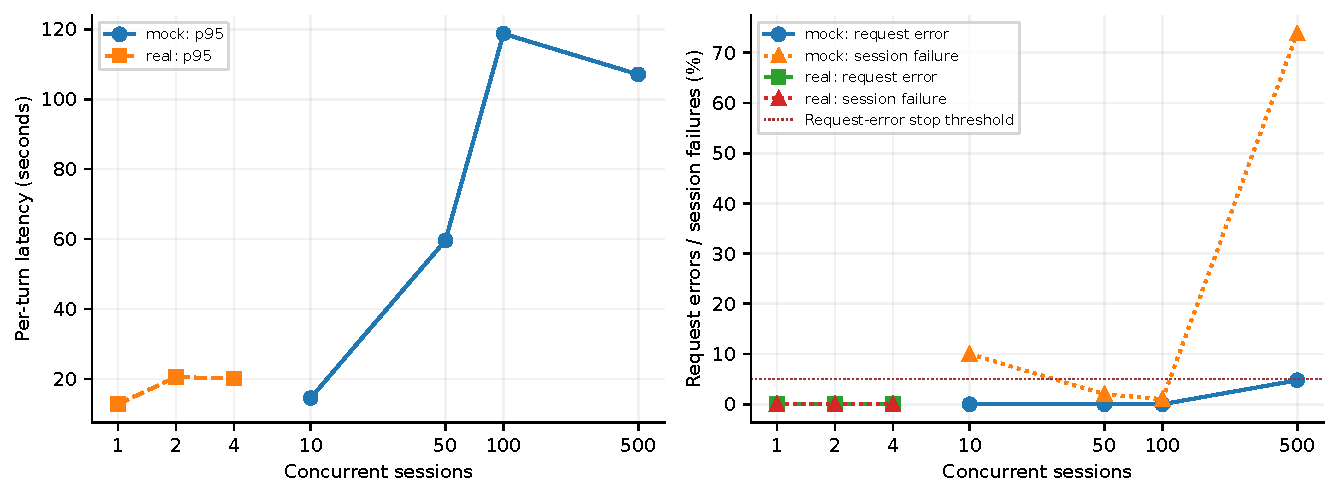
\includegraphics[width=\textwidth]{figures/fig_e4_load.pdf}
\caption{Local synthetic load experiment. Missing modes or levels were not
measured; the dotted line marks the declared early-stop threshold. Modes differ
in replay workload and backend revision.}
\label{fig:load}
\end{figure}

\section{Discussion}\label{sec:discussion}
The implementation demonstrates a concrete separation between questionnaire
control, model-assisted drafting, and EHR persistence. The principal contribution
is an inspectable contract and reproducible verification workflow. It is narrower
than a universally FHIR-native conversational agent: questionnaire source JSON
still controls the runtime, application-specific extensions carry additional
semantics, and internal calls use application contracts. These boundaries should
be explicit when adapting the framework to another institution.

Verification revealed issues that a successful end-to-end demonstration alone
would miss. Free-text EHR values cannot safely be forced into coded questionnaire
options. Conditional-semantic disagreement can discard information unless
detected, and validator failures can prevent an interoperability conclusion even
when a server accepts a transaction. Likewise, repeated synthetic sessions can
contaminate later inputs through prior write-backs. Recording these failures and
preserving their artifacts is necessary to distinguish repaired implementation
defects from limitations of the evaluation environment.

The simulated-patient harness also required verification. A substring-based
unknown-answer fallback could select a symptom option containing the same word
as an uncertainty label. Affected runs were excluded and preserved before a full
rerun with exact-option matching. This failure illustrates why API completion,
path agreement, and traceable chief-complaint facts cannot establish fidelity of
all subsequent simulated answers. Independent transcript review remains necessary.

The study cannot establish clinical safety, utility, or readiness for deployment.
Scenarios are author-drafted and await physician review; textual evidence matching
does not validate diagnostic interpretation; the simulated patient can still
hallucinate; and synthetic demographics do not reproduce local disease burden.
Only chief-complaint safety screening is active in the default workflow.
Questionnaire terminology and smoking-status mappings require clinical governance.
The local sandbox bypasses production authentication, and concurrency measurements
do not test multi-institution isolation, recovery, national networking, or the
national exchange hub. Model aliases may change upstream even when their reported
version strings are logged. Local model digests and prompt hashes improve
reproducibility but cannot make commercial inference fully deterministic.

The next acceptance steps are physician approval of scenario content and paths,
independent transcript and evidence audits, resolution of validator and terminology
gaps, and evaluation of the deployed authentication and EHR integration boundary.
Clinical effectiveness should be studied separately using an approved protocol;
it cannot be inferred from software completion or conformance rates.

\section{Conclusion}\label{sec:conclusion}
A modular pre-consultation implementation can make questionnaire control,
model configuration, provenance, and FHIR write-back inspectable and testable.
The present evidence supports a reproducible technical verification workflow,
with explicit failures and pending review. It does not establish diagnostic
accuracy, clinical safety, or national-scale deployment readiness.

\backmatter
\bmhead{Supplementary information}
The repository contains pinned versions, source-level synthetic-data mappings,
scenario review packets, model prompts and disclosure, raw run manifests,
audit samples, and generated tables. Table~\ref{tab:versions} lists principal
software versions; complete digests are in the machine-readable lock file.

\begin{table}[t]\centering
\caption{Principal pinned software versions. Model configurations and full
artifact digests accompany the experiment manifests.}
\label{tab:versions}\small
% Generated; edit source results or generator, never these values.
\begin{tabular}{ll}
\hline
Component & Pinned version \\[4pt]
\hline\noalign{\vskip 3pt}
Synthea & v4.0.0 \\[3pt]
FHIR & 4.0.1 \\[3pt]
HAPI image & hapiproject/hapi:v8.8.0-1 \\[3pt]
TW Core IG & 1.0.0 \\[3pt]
HL7 validator & 6.10.4 \\[3pt]
Python & 3.12.15 \\[3pt]
Node & v22.23.2 \\[3pt]
Ollama & 0.32.6 \\[3pt]
default extraction & gemini-3.6-flash \\[3pt]
default summary extraction & gemini-3.5-flash-lite \\[3pt]
default summary reasoning & gemini-3.6-flash \\[3pt]
Alternate Gemini & gemini-2.5-flash \\[3pt]
Local Gemma & gemma3:12b \\[3pt]
patient simulator model & qwen2.5:7b-instruct \\[3pt]
\hline
\end{tabular}

\end{table}

\bmhead{Acknowledgements}
Author confirmation of acknowledgements and institutional wording is pending.

\section*{Declarations}
\textbf{Funding.} Authors must supply and verify funding information.\par
\textbf{Competing interests.} Authors must provide their declarations.\par
\textbf{Ethics and consent.} These verification runs use synthetic data only.
No claim of institutional ethics approval or exemption is made; authors must
confirm the applicable institutional determination before submission.\par
\textbf{Data and code availability.} Scripts, configuration, derived summaries,
and asset generators are in the project repository. Large synthetic bundles
and raw local runs are regenerable and excluded from source control. A public
archival identifier and access statement require author confirmation.\par
\textbf{Author contributions.} Contributions and final approval require author
confirmation.\par
\textbf{Use of language models.} Language models assisted implementation,
synthetic scenario drafting, experiment orchestration, and manuscript preparation.
System and simulated-patient configurations, prompt hashes, and run dates are
recorded in \texttt{experiments/llm\_disclosure.json}. Physician scenario review
and transcript audits remain pending; no model output is represented as human
validation. Authors retain responsibility for source verification and the final
manuscript.

\bibliography{sn-bibliography}
